\section{Analizador de THD}
Se requiere diseñar un dispositivo de submetering que calcule en tiempo real
el THD de la tensión de línea de una subestación eléctrica. 

Para ello se ha de implementar el siguiente esquema:

\vspace{0.5cm}
\begin{figure}[H]
  \centering
  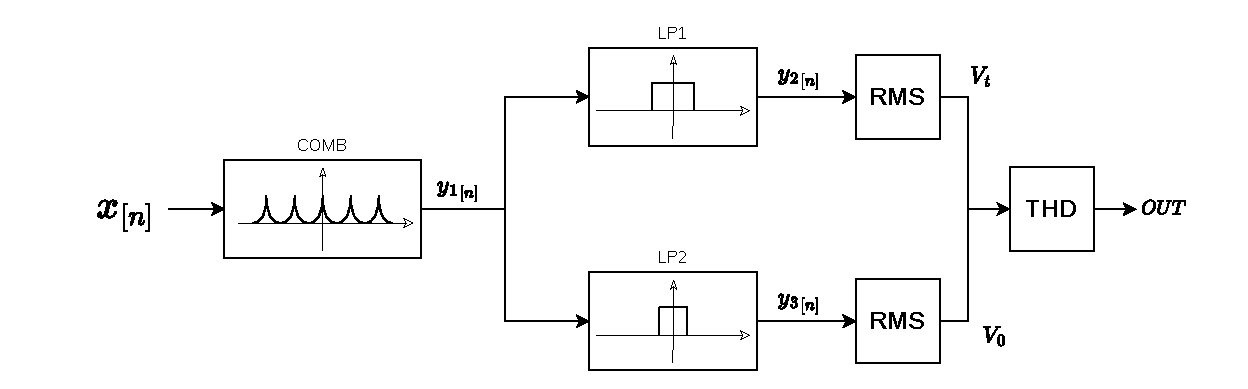
\includegraphics[width = \textwidth]{Imagenes/3_THD/esquema_THD.drawio.pdf}
  \caption{Esquema general a implementar.}
  \label{fig: esquema gral a implementar}
\end{figure}

\subsection{Diseño de bloques}
En este apartado se indicaran lass características de cada uno de los bloques enseñados en la figura \ref{fig: esquema gral a implementar} y se realizara el diseño de los mismos.

\subsubsection{Filtro comb}
Dado que se desea analizar los armónicos de la red, debemos de diseñar un filtro que disponga de ganancia unitaria para estos y las componentes restantes. En función de ello se solicita la característica de atenuar al menos 10 veces las frecuencias múltiplo impar de 25Hz. 

En vista de diseñar tal filtro, se dispone de la siguiente ecuación en diferencias:

\begin{equation}
y_1[n] = \alpha x[n] + \beta y_1[n-k]
\end{equation}

\noindent donde hemos de determinar $\alpha$, $\beta$ y $k$. Para ello podemos realizar un análisis desde la función transferencia del sistema:

\begin{equation}
    H_{(z)} = \frac{{Y_1}_{(z)}}{{X}_{(z)}} = \frac{\alpha}{1-\beta z^{-k}} = \frac{\alpha \cdot z^k}{z^k-\beta}
\end{equation}

\noindent donde resulta evidente que se dispone de k ceros en el origen y k polos repartidos uniformemente en una circunferencia de radio $\beta^{1/k}$. De este modo, k ha de corresponder con la cantidad de armónicos de 50Hz que entran en $f_s = 10kHz$; de este modo, k=200. Luego debemos de ajustar $\alpha$ y $\beta$ tal de obtener las ganancias deseadas. En función de ello se puede analizar la respuesta en frecuencia del sistema:

\begin{align*}
    |H_{(\omega)}| = \frac{\alpha}{\sqrt{(cos(\omega k) - \beta)^2 + sen^2(\omega k)}} = \frac{\alpha}{\sqrt{1 + \beta^2  - 2 \cdot \beta \cdot cos(\omega k)}} = 
\end{align*}

\noindent de este modo, la ganancia en los picos esta dada cuando $\omega = 2\pi / k$, tal que:

\begin{equation}
    \frac{\alpha}{1-\beta} = 1 \Longrightarrow \alpha = 1-\beta
\end{equation}

\noindent mientras que los múltiplos impares de 25Hz corresponden a $\omega = \frac{2\pi \cdot m \cdot 25Hz}{2\pi \cdot f_s} = m \cdot \frac{\pi}{k}$ con m impar. Por ende:

\begin{equation}
    \frac{\alpha}{1+\beta} = 0.1 \Longrightarrow \alpha = 0.1 + 0.1\beta
\end{equation}

\noindent resolviendo el sistema de ecuaciones se obtiene $\alpha = 2/11$ y $\beta = 9/11$.